% !TEX program = xelatex

\documentclass[12pt, a4paper]{article}

\usepackage{fontspec}
\setmainfont[Ligatures=TeX]{Linux Libertine O}

\usepackage[hidelinks, colorlinks = true, urlcolor = blue]{hyperref}
\usepackage{indentfirst}
\usepackage{graphicx}
\usepackage[left=2cm,right=2cm,top=2.5cm,bottom=2.5cm]{geometry}
\usepackage{lipsum}

%\setlength{\parindent}{1em}
%\setlength{\parskip}{1em}\title{Εργασία Στατιστικής}

%\title{Java socket programming \\ 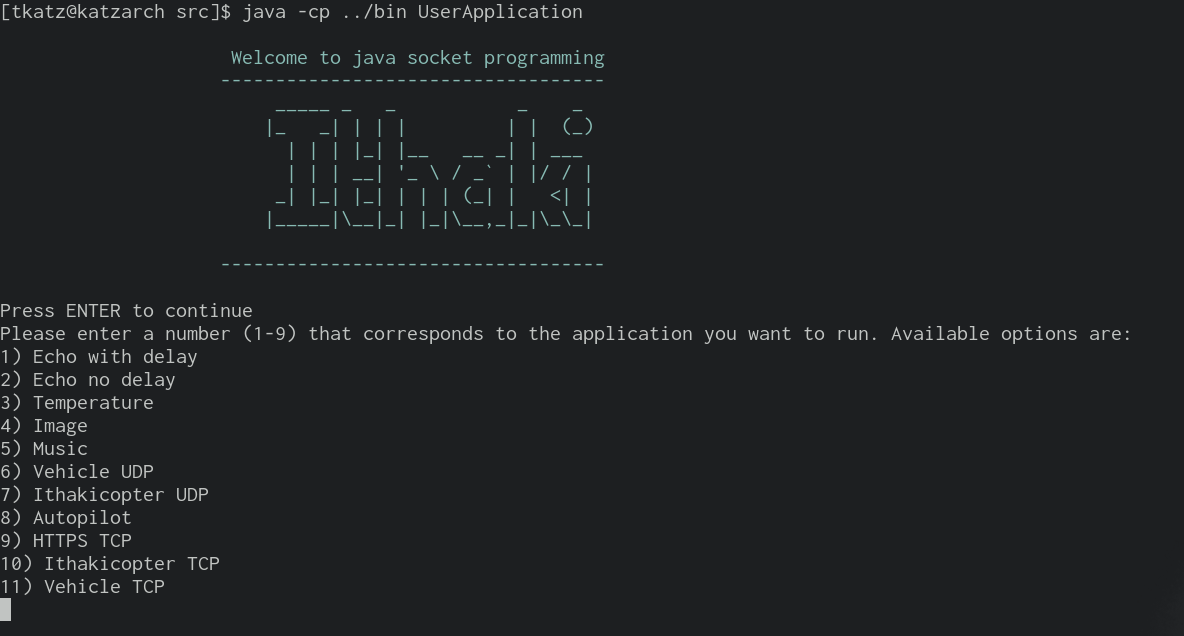
\includegraphics[width=\textwidth]{assets/login.png}}
% \author{Θεόδωρος Κατζάλης \\ ΑΕΜ:9282 \\ katzalis@auth.gr}
% \date{19/07/2020}

\begin{document}

\begin{titlepage}

\begin{figure}[h!]
  \begin{center}
    
\includegraphics[width=3cm]{assets/auth.pdf}
    \label{fig:cover_auth_logo}
  \end{center}
\end{figure}

\centering
\Large Αριστοτέλειο Πανεπιστήμιο Θεσσαλονίκης\\
\Large Πολυτεχνική Σχολή\\
%\large Τμήμα Ηλεκτρολόγων Μηχανικών και Μηχανικών Υπολογιστών\\
%\large Τομέας Τηλεπικοινωνιών

\vspace{\fill}

\LARGE \textbf{Java socket programming} \\
\LARGE \textbf{Δίκτυα 2}

\vspace{\fill}

\Large Θεόδωρος Κατζάλης \\
\Large ΑΕΜ:9282 \\ 
\Large katzalis@auth.gr

\vspace{\fill}
\raggedright

\centering
\vspace{\fill}
\today

\end{titlepage}

%\maketitle


\pagebreak
\tableofcontents
%\pagebreak

% \section{Lorem}
% \lipsum


\section{Ρυθμίσεις router}


\begin{figure}[h!]
\centering
	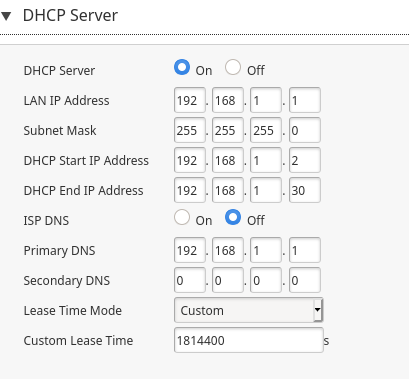
\includegraphics[height=.3\textheight, width=\textwidth, keepaspectratio]{assets/router/dhcp.png}
	\caption{DHCP} 
    \label{fig:dhcp}
\end{figure}




\begin{figure}[h!]
\centering
	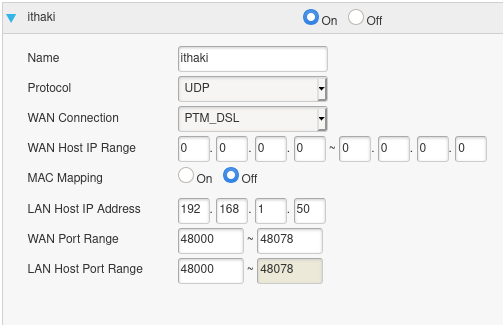
\includegraphics[height=.3\textheight, width=\textwidth, keepaspectratio]{assets/router/port_forwarding.png}
	\caption{Port forwarding} 
    \label{fig:portforward}
\end{figure}


\pagebreak
\begin{figure}[h!]
\centering
	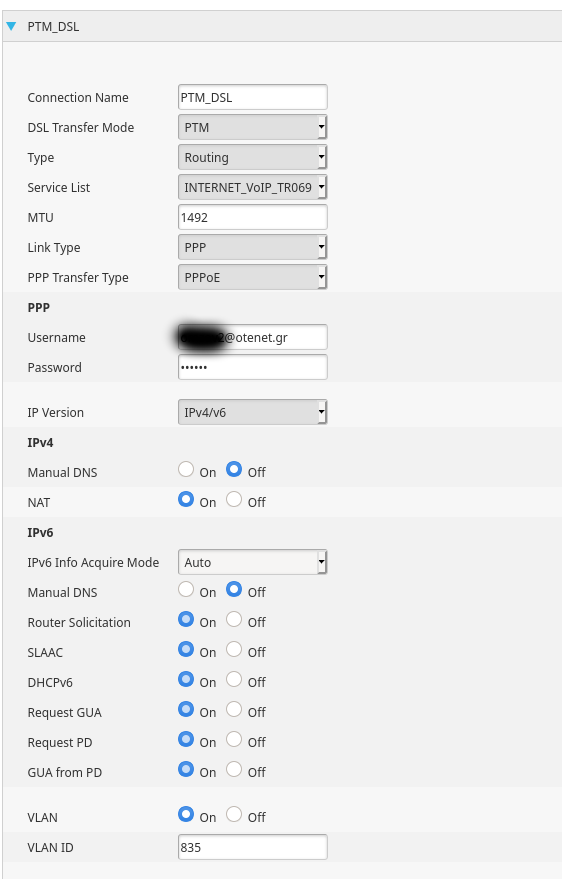
\includegraphics[height=.75\textheight, width=\textwidth, keepaspectratio]{assets/router/authentication.png}
	\caption{Authentication: User is registered} 
    \label{fig:auth}
\end{figure}

\begin{figure}[h!]
    \centering
    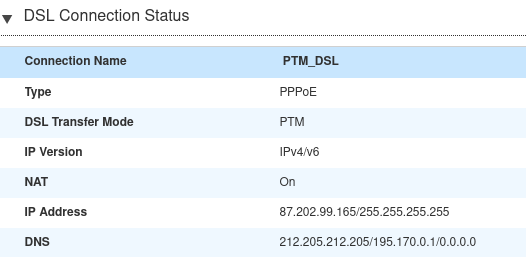
\includegraphics[height=.3\textheight, width=\textwidth, keepaspectratio]{assets/router/public.png}
    \caption{Public IP address (χωρίς CGNAT)} 
    \label{fig:publicip}
\end{figure}

\pagebreak
\section{Ρύθμιση private static IP}

Σχόλιο: Η static IP address πρέπει να είναι εκτός του DHCP range, για να αποφύγουμε τυχόν conflict σε περίπτωση που ο DHCP server αποφασίσει να δώσει IP ίδια με αυτήν που έχουμε ορίσει ως στατική.

\begin{figure}[h!]
    \centering
    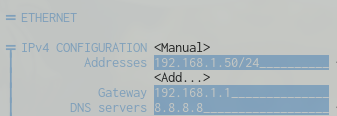
\includegraphics[height=.3\textheight, width=\textwidth, keepaspectratio]{assets/router/static.png}
    \caption{Setting static IP address via network manager. Ethernet interface} 
    \label{fig:static}
\end{figure}

\end{document}
